\chapter{Implementation} \label{chap:implementation}

\section*{}

\section{Methodology} \label{sec:meth}

Like any software development project, a simulation project also has a life 
cycle. In this section we describe the steps to apply in the simulation 
methodology, based on Ulgen et al.~\cite{Ulgen1994} and Banks et 
al.~\cite[section 1.11]{Banks2004}, which can be summarized as follows:

\begin{enumerate}
    \item \textit{Problem formulation}: Clear statement of the problem by the 
    analyst and stakeholders; \label{enum:mform}
    \item \textit{Setting of objectives and overall project plan}: Questions to 
    be answered by the simulation, plans for the study, cost and number of days 
    for each phase, with the results expected at each stage; \label{enum:mobj}
    \item \textit{Model conceptualization}: Select, modify and iterate over the 
    assumptions that characterize the system; \label{enum:mconcept}
    \item \textit{Data collection}: Collect the necessary data to run and 
    validate the model, assuming that required data will change with the 
    increasing complexity of the system; \label{enum:mdata}
    \item \textit{Model translation}: Materialization of the system in a 
    program; \label{enum:mtransl}
    \item \textit{Verification}: Making sure that the program behaves correctly 
    accordingly to its inputs; \label{enum:mverif}
    \item \textit{Validation}: Calibration of the model, comparing the model 
    against an actual system; \label{enum:mvalid}
    \item \textit{Experimental design}: Tweak the experiments, comparing 
    alternative designs; \label{enum:mexp}
    \item \textit{Production runs and analysis}: Estimate measures of 
    performance for the systems that are being simulated; \label{enum:mprod}
    \item \textit{Documentation and reporting}: Document both the program and 
    the progress of the study; \label{enum:mdocs}
    \item \textit{Implementation}: End result of the study, including the 
    entire simulation process. \label{enum:mimpl}
\end{enumerate}

This process can be visualized in figure \ref{fig:sim}.

\begin{figure}[h]
    \begin{center}
        \leavevmode
        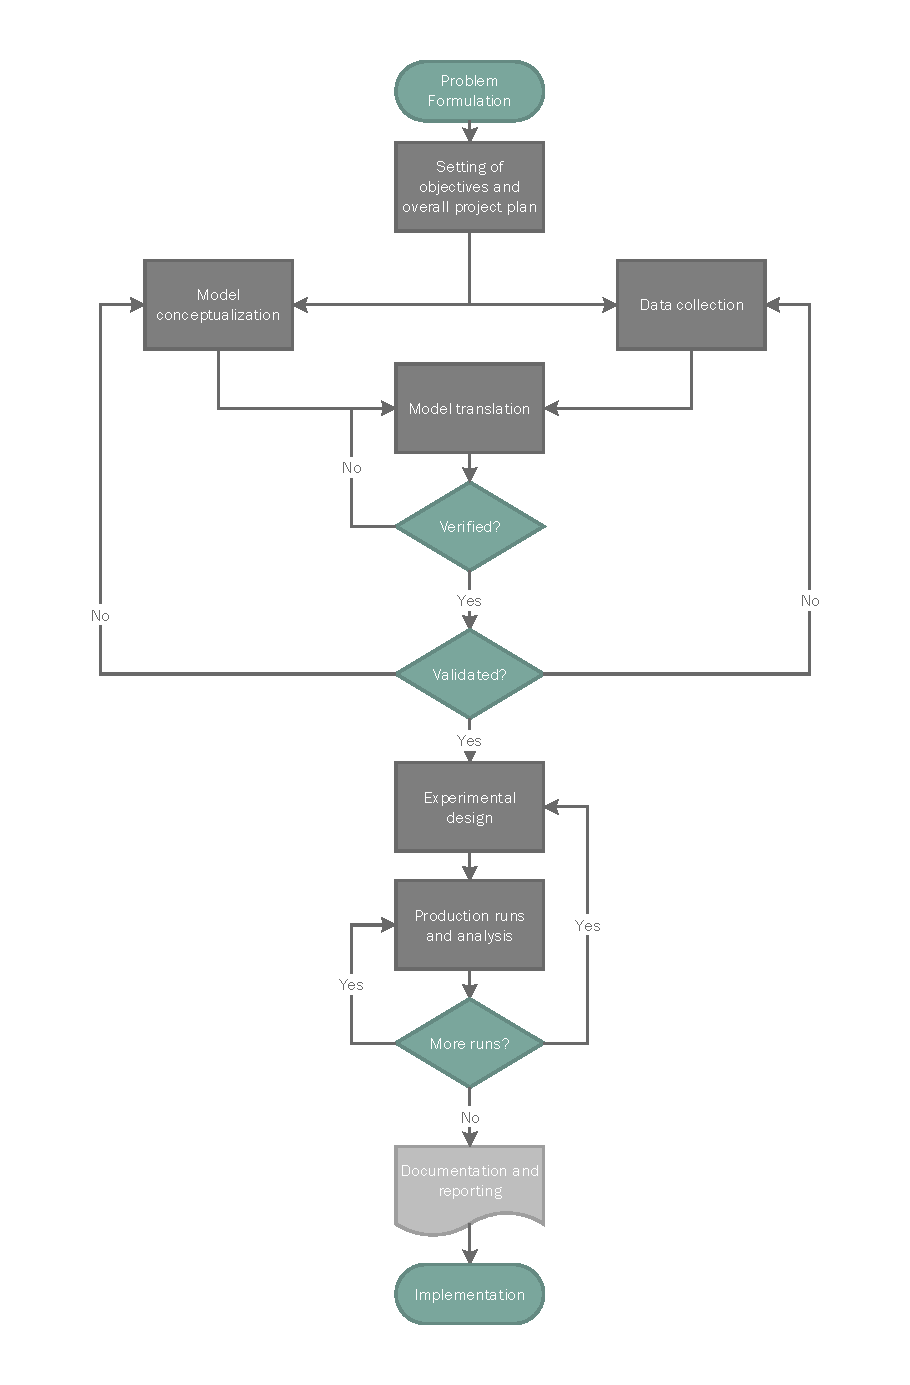
\includegraphics[width=0.6\textwidth]{simulation_study}
        \caption{Steps in a simulation study \cite{Banks2004}}
        \label{fig:sim}
    \end{center}
\end{figure}

\section{Requirements}

\subsection{Website Representation}
\subsection{Navigation Agents}
\subsection{Recommendation Agents}
\subsection{Simulation Engine}
\subsection{Reporting}

\section{Architecture}

\subsection{Physical Architecture}
\subsection{Logical Architecture}
\subsection{Class Architecture}

\begin{figure}[h]
    \begin{center}
        \leavevmode
        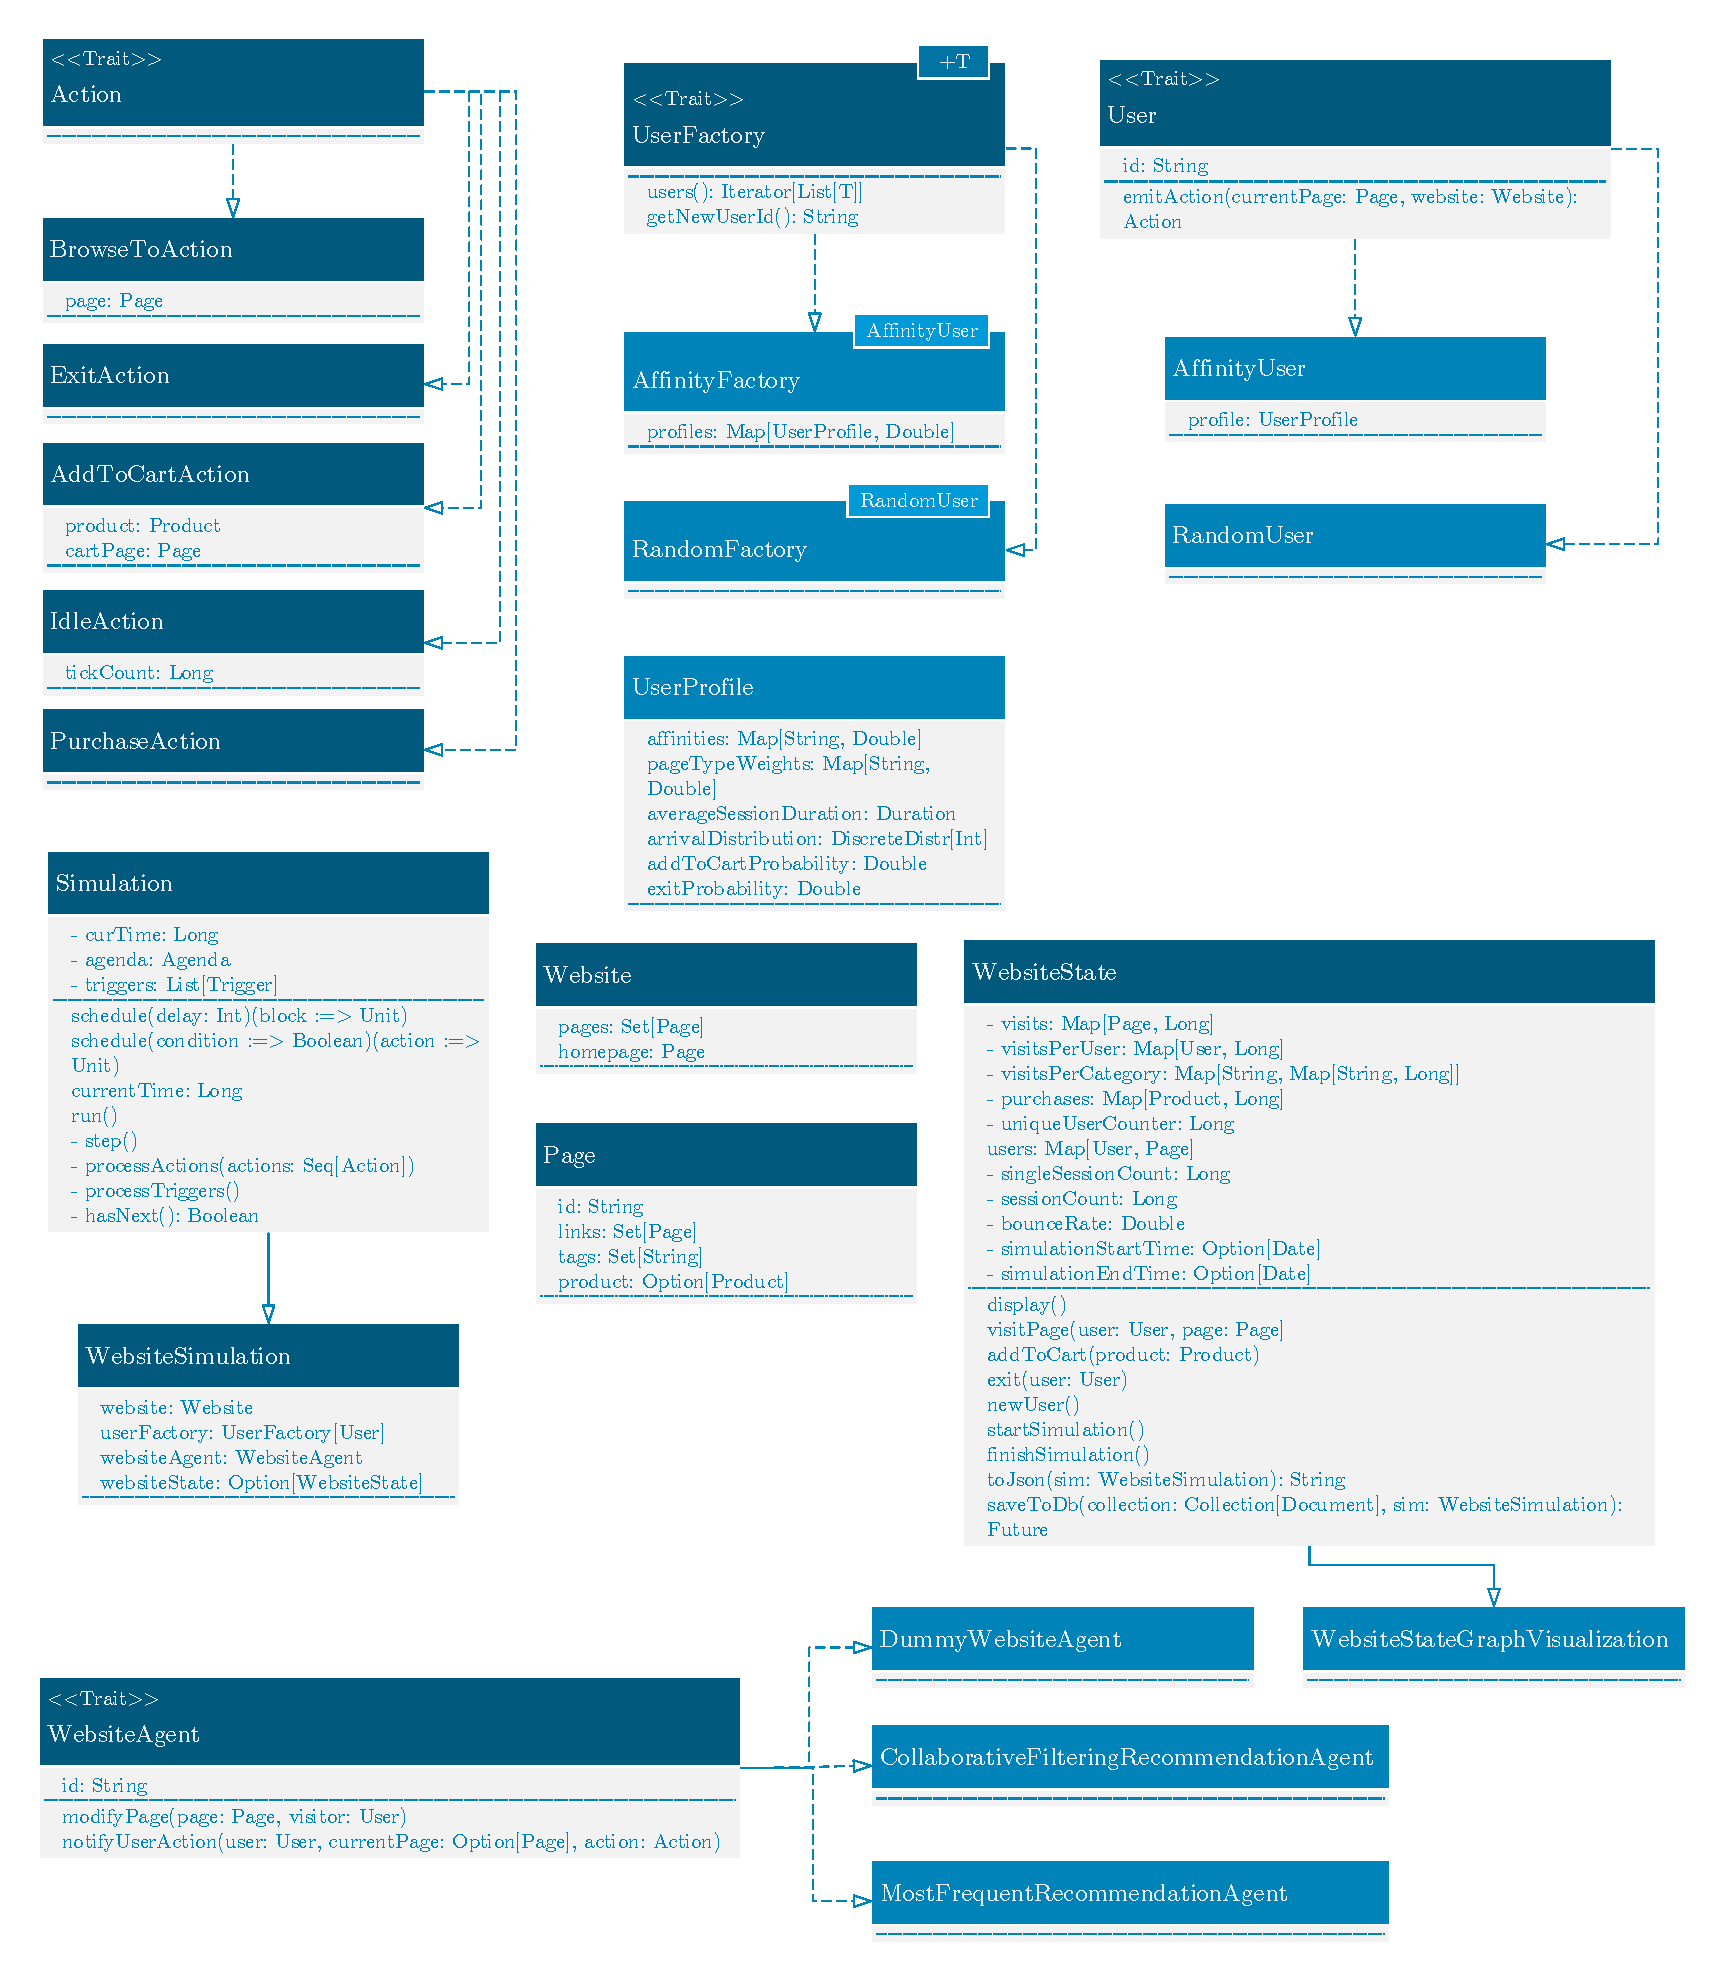
\includegraphics[width=0.95\textwidth]{class_diagram}
        \caption{Class diagram}
        \label{fig:class}
    \end{center}
\end{figure}

\subsection{Agent Architecture}
\subsection{Interface}

\section{Technology}
